%ullright document template
%default a4 one-sided article page setup
\documentclass[article, a4paper, oneside, 11pt]{memoir}

%the following three commands are necessary when using pdflatex
%(set input/output encoding)
\usepackage[utf8]{inputenc}
\usepackage[T1]{fontenc}
\usepackage{helvet}
%use sans serife font for body 
\renewcommand*\familydefault{\sfdefault}

%but with more tech-doc like margins
\setlrmarginsandblock{2.8cm}{2.8cm}{*}
\checkandfixthelayout

%for the german language
\usepackage[ngerman]{babel}

%including pictures
\usepackage{graphicx}
\graphicspath{{./figures/}}

%wrapping text around figures
\usepackage{wrapfig}

%provides symbols for shift, enter, etc.
\usepackage{keystroke}

%url handling
\usepackage{url}

%elaborate references
\usepackage[ngerman]{varioref}

%we do not use xelatex anymore
%allows convenient font/color specification
%\usepackage{xcolor}
%\usepackage{fontspec}
%'classic' tex mappings, e.g. -- => en-dash
%\defaultfontfeatures{Mapping=tex-text}
%\setromanfont{Gentium Basic}
%\definecolor{DocBlue}{rgb}{0.1, 0.42, 0.59}
%\setsansfont[Color = DocBlue]{Ubuntu}

%enables pdf linking and attributes
\usepackage{hyperref}
\hypersetup{
    colorlinks=true,%
    citecolor=black,%
    filecolor=black,%
    linkcolor=black,%
    urlcolor=black,%
    pdfauthor={ull.at},%
    pdftitle={ullright Handbuch},%
    pdfsubject={ullright}
}

\chapterstyle{veelo}
\headstyles{komalike}
\pagestyle{empty}

%header and footer images on every page
\usepackage{wallpaper}
\ULCornerWallPaper{1.0}{header}
\LLCornerWallPaper{1.0}{footer}

%Precise figure placement
% \usepackage{float}

%padding for fbox borders
%\setlength\fboxsep{0pt}

%color headlines
\usepackage{color}
\usepackage{titlesec}

\definecolor{ullblue}{rgb}{0.1, 0.42, 0.59}

\titleformat{\chapter}[display]
{\color{ullblue}\normalfont\huge\bfseries}{\chaptertitlename\
\thechapter}{20pt}{\Huge}

\titleformat{\section}
{\color{ullblue}\normalfont\Large\bfseries}{\thesection}{1em}{}

% Do not indent paragraphes but add newlines
\usepackage{parskip}
\setlength{\parindent}{0cm}
\setlength{\parskip}{2mm}


%memoir recommendation
\clubpenalty=10000
\widowpenalty=10000
\raggedbottom


\begin{document}

\vspace*{3cm}
%move picture left/right
\begin{figure}[htp]
\centering

\includegraphics[width=0.5\textwidth]{softwarebox}
\end{figure}

\vspace{3cm}

%we do not use xelatex anymore
{%\fontspec[Scale=1.4, Color = DocBlue]{Ubuntu Bold}
\LARGE
\color{ullblue}
ullright -- Plattform für Enterprise 2.0 Webapplikationen
}

\vspace{0.2cm}

{%\fontspec[Scale=1.4, Color = DocBlue]{Ubuntu Bold}
\large
%\color{ullblue}
%Ein Modul der ullright-Plattform -- www.ullright.org
}

\vspace{1cm}

%we do not use xelatex anymore
{%\fontspec[Scale=0.8]{Gentium Basic}
\footnotesize
27.04.2010 -- Martin Leonhartsberger-Schrott

24.02.2010 -- Klemens Ullmann-Marx
}

\clearpage

\pagestyle{plain}

%\setcounter{page}{1}

%number and include in toc up until subsections
\setcounter{secnumdepth}{2}
\setcounter{tocdepth}{2}
\tableofcontents*

\clearpage

\addtocounter{chapter}{1}

%the star prevents this chapter from being added to the toc and from being numbered
\chapter*{ullright}

\section{Einleitung}
ullright ist eine Plattform für Enterprise 2.0 Webapplikationen. Das Projekt steht unter der Leitung der Firma ull.at und wird als OpenSource Community-Projekt entwickelt.

Die Zielgruppe von ullright sind mittelständische Unternehmen die Ihre internen Abläufe durch einfach zu bedienende und gut integrierte Webapplikation unterstützen möchten.

ullright bietet fertige Module wie zum Beispiel ullWiki, ullFlow oder ullVentory. Diese Module bieten eine Vielzahl von Grundfunktionen und lassen sich bei Bedarf leicht anpassen und erweitern.

Ausführliche Informationen zu den Modulen finden Sie in den entsprechenden Handbüchern.

ullright fungiert aber auch als Entwicklungsplattform für individuelle Anwendungen. Individualentwicklungen lassen sich rasch und kostengünstig umsetzen, da bereits eine Vielzahl an wiederverwendbaren Komponenten zur Verfügung stehen. Dies erlaubt auch die Migration bestehender Anwendungen (Stichwort "`Wildwuchs"') auf eine gemeinsame, stabile und gemanagte Plattform.

Die Bedienung erfolgt über eine übersichtliche und einfach zu bedienende Weboberfläche. Daraus ergibt sich ein geringer Einschulungsaufwand und eine hohe Akzeptanz durch die Mitarbeiter. Auch die Möglichkeit  kundenspezifischer Anpassungen trägt zur optimalen Unterstützung der Mitarbeiter und Abläufe bei.

ullright bietet eine Vielzahl an Möglichkeiten für Schnittstellen um das System optimal in die bestehende IT-Landschaft zu integrieren. Bespiele: Active Directory, Lotus Notes, HR-Systeme und alle anderen Systeme die offene Schnittstellen bieten. Dadurch ist es möglich die Duplikation von bespielsweise Benutzerdaten oder Passwörtern zu vermeiden.

\subsection{Systemvoraussetzungen}
\begin{itemize}
\item Cookies müssen aktiviert sein
\item Wir empfehlen einen aktuellen Browser zu verwenden (Firefox 3.5, Internet Explorer 8, ...)
\item Javascript ist keine Voraussetzung, wird aber für eine einfachere Benutzeroberfläche empfohlen.
\end{itemize}
\section{Aufbau}
\subsection{Architektur}
"`ullright"' ist der Überbegriff für die in Abbildung \vref{fig:platform} gezeigte Plattform.

\begin{figure}[htp]
\centering
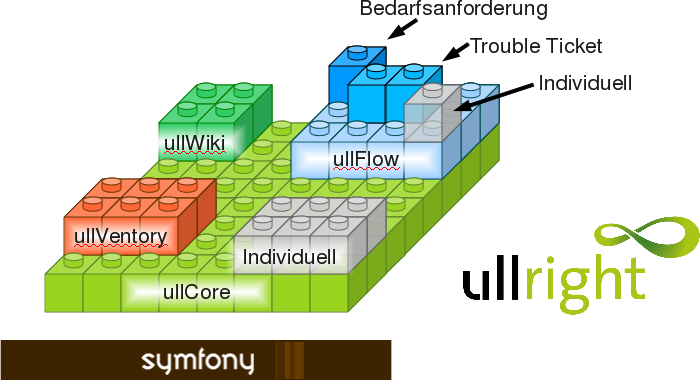
\includegraphics[width=0.9\textwidth]{figures/ullrightgermanexport-img2.png}
\caption{Die ullright-Plattform}
\label{fig:platform}
\end{figure}

Aufbauend auf einer Webserviceinfrastruktur bestehend aus Webserver und Datenbank besteht die Plattform ullright aus folgenden Komponenten:

\begin{enumerate}
\item Symfony PHP5 Framework
\item ullCore Basismodul
\item Module
\begin{itemize}
\item Generische Module -- Zum Beispiel ullWiki, ullVentory, \ldots
\item Individuelle Module
\end{itemize}
\end{enumerate}
\subsection{Module}
Die einzelnen Module nutzen die Infrastruktur des ullCore Basismoduls. Gemeinsam ist allen Modulen eine ähnlich aufgebaute Benutzeroberfläche, damit Sie sich rasch zurechtfinden.

Die Module sind getrennt installierbar.

Zur besseren Unterscheidung der einzelnen Module hat jedes Modul eine eigenes Farbschema:

\begin{enumerate}
\item Basiskomponenten und Administration: grau
\item ullWiki: grün
\item ullFlow: blau
\item ullVentory: orange
\end{enumerate}
\subsection{Seitenaufbau der Weboberfläche}

\begin{figure}[htp]
\centering
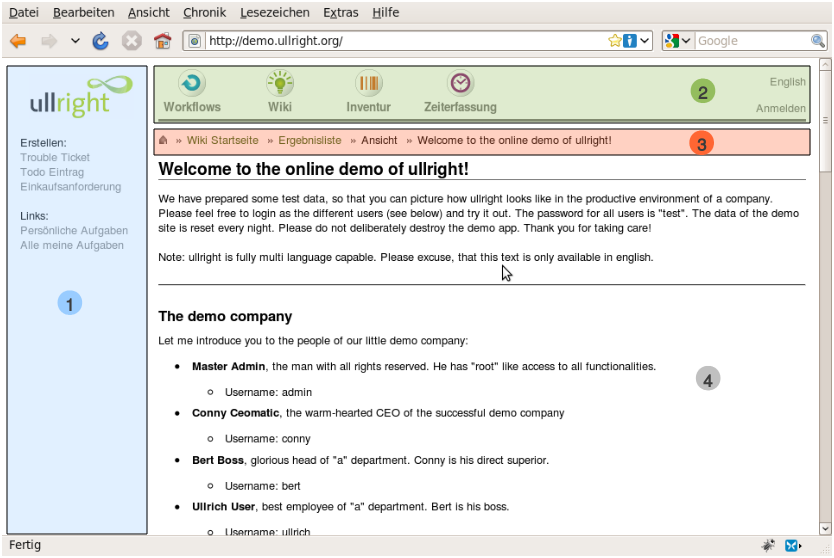
\includegraphics[width=0.9\textwidth]{figures/ullrightgermanexport-img3.png}
\caption{Eine typische ullright-Seite}
\label{fig:typical_page}
\end{figure}
Jede Seite setzt sich aus den gleichen Elementen zusammen, die in Abbildung \vref{fig:typical_page} ersichtlich sind:

\begin{enumerate}
\item Sidebar (Seitenleiste)
\item Hauptnavigation
\item Breadcrumbs\footnote{In Anlehnung an die verstreuten Brotkrumen im Grimm-Märchen "`Hänsel und Gretel"'.  Siehe auch http://de.wikipedia.org/wiki/Brotkrumennavigation} (Brotkrumennavigation)
\item Inhalt (Contentbereich)
\item Fußzeile (nicht auf der Abbildung ersichtlich)
\end{enumerate}
\subsection{Sidebar}
In der Sidebar befinden sich häufig benutzte Funktionen und Links. In Abhängigkeit des aktiven Moduls kann sich der Inhalt der Sidebar dynamisch ändern. Der Sidebar können auf Wunsch auch individuelle Funktionen und Links hinzugefügt werden.

\subsection{Hauptnavigation}
Die Hauptnavigation beinhaltet folgende Elemente:

\begin{description}
\item[Modulicons] Alle aktivierten ullright Module sind hier mit dem jeweiligen Icon vertreten. Beispiele: ullWiki, ullVentory, Administrationsbereich. Hinweis: manche Icons werden nur mit entsprechenden Zugriffsrechten angezeigt. Auf Wunsch können individuelle Icons hinzugefügt werden.
\item[Sprachauswahl] Falls mehrere Sprachen aktiviert sind, können Sie hier die Sprache wählen.
\item[Anmeldung] Hier wird entweder der Link zur Anmeldung angezeigt, oder wenn man bereits angemeldet ist der Benutzername und der Link zur Abmeldung.
\end{description}
\subsection{Breadcrumbs}
Die Breadcrumbleiste zeigt den Pfad zur aktuell gezeigten Seite. Sie erlaubt den schnellen Überblick wo man sich befindet. Außdem ermöglicht die Breadcrumbleiste zum Beispiel von der Bearbeitunsseite mit einem Klick zur Modul-Startseite oder zur Listenansicht zu wechseln.

Erklärung des Beispiels aus der Abbildung "`Seitenaufbau"' oben:

\begin{itemize}
\item Über das "`Haus"'-Icon gelangen Sie zur ullright Startseite. Es symbolisiert den Beginn des Pfades.
\item "`Wiki Startseite"' zeigt Ihnen das aktuelle Modul an und erlaubt Ihnen ein rasches Wechseln zur Modul-Startseite.
\item Über den Link "`Ergebnisliste"' gelangen Sie zur Listenansicht des Modules
\item "`Ansicht"' - Sie befinden sich gerade im Ansichtsmodus und zwar betrachten Sie das Dokument "`Welcome to the online demo of ullright!"'
\end{itemize}
\subsection{Inhalt}
Hier wird der Inhalt der aktuellen Seite angezeigt

\subsection{Fußleiste}
Die Fußleiste enthält die Copyrightinformationen und Links zum Hersteller und zur Projektseite.

\section{Anmeldung}
Für viele Funktionen in ullright ist eine Anmeldung erforderlich damit das System überprüfen kann welche Rechte der Benutzer hat.

\begin{figure}[htp]
\centering
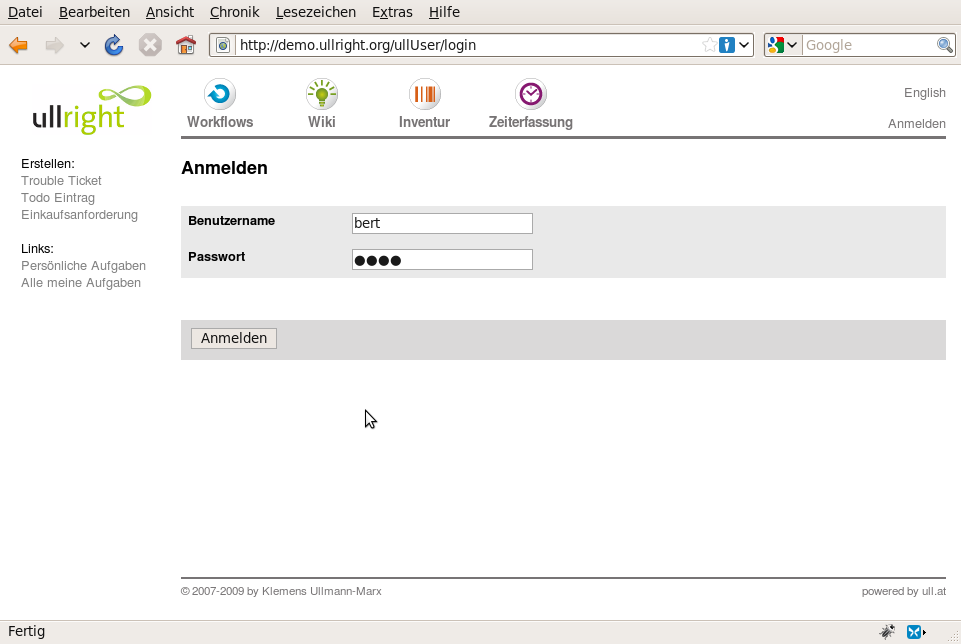
\includegraphics[trim=0 250pt 0 0,clip,width=0.9\textwidth]{figures/ullrightgermanexport-img4.png}
\caption{Die Anmeldeseite}
\label{fig:login}
\end{figure}

Klicken Sie in der Hauptnavigation auf "`Anmelden"'.

Geben Sie nun Ihren Benutzernamen und Ihr Passwort ein und klicken Sie auf den Button "`Anmelden"' (siehe Abbildung \vref{fig:login}).

Wenn die Anmeldung erfolgreich war, werden Sie automatisch zur ursprünglichen Seite weitergeleitet. Zudem sehen Sie nun in der Hauptnavigation, daß Sie z.B. als Benutzer "`Bert"' angemeldet sind.

\section{Sprachauswahl}
Ebenfalls in der Hauptnavigation befindet sich die Sprachauswahl. Standardmäßig wird ullright in den Sprachen Deutsch und Englisch ausgeliefert. ullright erkennt die Sprache Ihres Webbrowsers und wählt automatisch die passende Sprache. 

Wenn Sie eine andere Sprache verwenden möchten wähle Sie diese bitte aus.

Auf Wunsch können weitere Sprachen hinzugefügt werden.

\section{Erweiterte Suche}
Die erweiterte Suche erlaubt komplexe benutzerdefinierte Abfragen. Sie funktioniert für alle ullright Module gleich und unterscheidet sich nur durch die zur Verfügung stehenden Kriterien.

Wir behandeln als Beispiel die erweiterte Suche der Benutzerverwaltung, siehe Abbildung \vref{fig:advanced_search}.

(Klick auf "`Admin"' in der Hauptnavigation, dann auf "`Erweiterte Suche"')


\begin{figure}[htp]
\centering
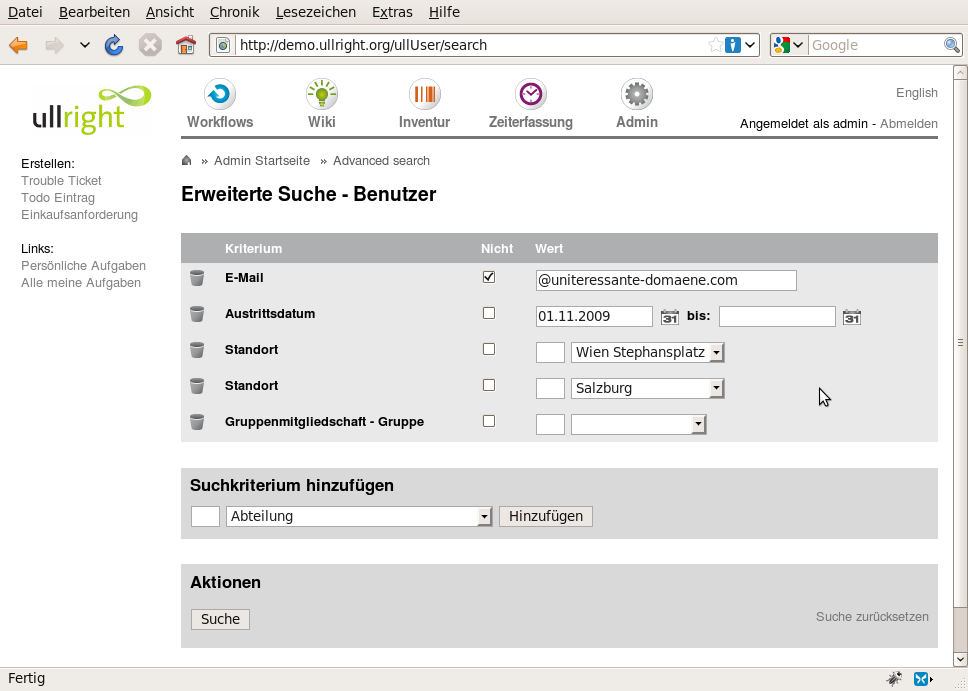
\includegraphics[width=0.9\textwidth]{figures/ullrightgermanexport-img5.png}
\caption{Die erweiterte Suche}
\label{fig:advanced_search}
\end{figure}


\subsection{Kritierien}
Die Liste der Kriterien stellt den obersten Bereich dar. Hier werden alle hinzugefügten Kriterien mit den dazugehörigen Suchfeldern angezeigt.

Je nach Feldtyp (Text, Auswahlfeld, Datum) werden unterschiedliche Suchfelder angezeigt.

\paragraph{Kriterium löschen}
Das Papierkorbsymbol löscht ein Kriterium aus der Liste.

\paragraph{Verneinung}
Das "`Nicht"' Ankreuzfeld verneint das Suchfeld. Im allgemeinen Sprachgebrauch entspricht dies dem "`außer"'. Beispiel: Suche alle E-Mailadressen außer denen die "`@uninteressante-domaene.com"' enthalten.

\paragraph{Feldtyp Text}
Bei Texteingabefeldern können Sie einfach beliebige Suchbegriffe eingeben. Standardmäßig wird eine sogenannte unscharfe Suche verwendet, die vorne und hinten Wildcards\footnote{Zu Deutsch "`Platzhalter"' oder "`Joker"'} hinzufügt. Beispiel: "`right"' findet auch "`ullright"'.

Wenn Sie genauer suchen möchten können Sie die scharfe Suche aktivierten in dem Sie den Begriff in doppelte Anführungszeichen stellen.

\paragraph[Feldtyp Auswahlliste]{Feldtyp Auswahlliste}
Bei Auswahlboxen müssen Sie nur den gewünschten Eintrag aus der Liste auswählen

\paragraph{Feldtyp Datum und Zahlen}
Bei Datumsfeldern und Zahlenfeldern steht Ihnen eine "`Von -- Bis"' Suche zur Verfügung.

Damit können Sie nach Intervallen suchen. Beispiel: alle Benutzer die zwischen dem 1.Jänner 2009 und dem 31.Juni 2009 ausgetreten sind.

Sie können eines der Felder leer lassen. Wenn Sie das "`von"' Feld leer lassen werden alle Einträge bis zum gegebenen Datum gefunden. Wenn Sie das "`bis"' Feld leer lassen werden alle Einträge ab dem eingegebenen "`von"' Datum gefunden.

\paragraph{Feldtyp Ankreuzfeld (Checkbox)}
Ankreuzfelder werden in der erweiterten Suche als Auswahllisten angezeigt. Wählen Sie "`Ja"' oder "`Nein"' aus für "`angekreuzt"' bzw "`nicht angekreuzt"'.

\paragraph{Mehrfachauswahl}
Beispiel: Sie möchten alle Benutzer der Standorte Wien und Salzburg anzeigen lassen.

Fügen Sie dazu zwei Mal das Kriterium Standort hinzu und wählen Sie einmal Wien und einmal Salzburg aus.

\paragraph{Leere Kriterien}
Wenn Sie das Suchfeld eines Kriteriums leer lassen wird es einfach nicht beachtet.

\subsection{Suchkriterium hinzufügen}
Wählen Sie die gewünschten Kriterien aus der Liste aus und klicken Sie auf "`Hinzufügen"'.

\subsection{Suche starten}
Wenn Sie mit der Auswahl der Kriterien und dem Eintragen der Suchbegriffe fertig sind klicken Sie auf "`Suche"' um die Suche zu starten

\section{Feldtypen und deren Optionen}
In manchen Modulen (ullFlow, ullVentory) können Sie über die Weboberfläche Felder hinzufügen.

Dabei ist jeweils die Eingabe eines Feldtyps (z.B. Datum) und falls nötig von Optionen notwendig.

Die Optionen werden im Format "`\texttt{option1=wert1 option2=wert2}"' (getrennt durch Leerzeichen, ohne Anführungszeichen) angegeben, siehe dazu Abbildung \vref{fig:field_options}.

\begin{figure}[htp]
\centering
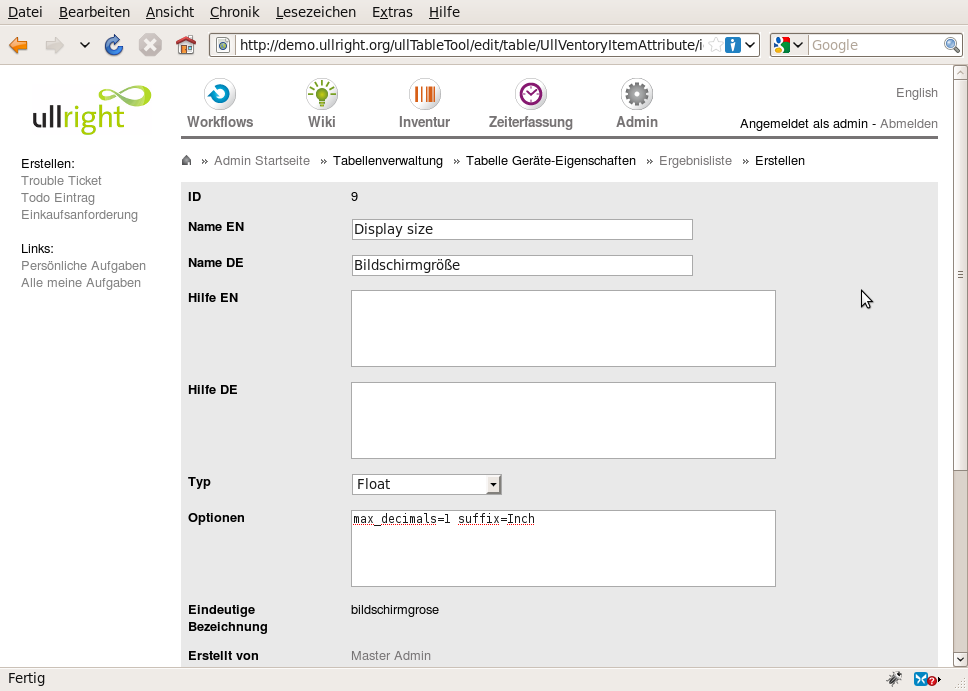
\includegraphics[width=0.9\textwidth]{figures/ullrightgermanexport-img6.png}
\caption{Eingabe von Feldtypen-Optionen}
\label{fig:field_options}
\end{figure}

Hier die Liste der verfügbaren Feldtypen und gegebenenfalls deren Optionen:

\subsection[Caller -- Benutzerauswahlfeld mit Link zu Inventory und Visitenkarte]{Caller -- Benutzerauswahlfeld mit Link zu Inventory und Visitenkarte}
\subsection{Checkbox -- Ankreuzfeld}
\subsection{Country - Landauswahl}
\subsection{Date -- Datum}
\subsection{Datetime -- Datum und Zeit}
\subsection{E-Mail}
\subsection{Float -- Dezimalzahl}
\begin{itemize}
\item max\_decimals -- Anzahl der Kommastellen (Ganzzahl)
\item suffix -- Einheit z.B. "`Ghz"' (Text)max\_decimals -- Anzahl der Kommastellen (Ganzzahl)
\end{itemize}
\subsection{IP address -- IP-Adresse}
\subsection{Information update -- Informationsaktualisierung}
Speichert den Verlauf einer Kommunikation ab. Wird für mehrzeilige Textfelder verwendet, wo der jeweilige Original-Inhalt nicht verändert werden soll. Einsatzbeispiel: Trouble Ticket

\subsection{Integer - Ganzzahl}
\begin{itemize}
\item suffix -- Einheit z.B. "`Ghz"' (Text)
\end{itemize}
\subsection{MAC adress -- MAC-Adresse}
\begin{itemize}
\item Eindeutige Hardwareadresse von Netzwerkgeräten
\end{itemize}
\subsection{Password -- Passwort}
\subsection{Percentage -- Prozentsatz}
Grafischer Schieberegler. Einsatzbeispiel: Fortschritt einer Aufgabe

\begin{itemize}
\item min -- Minimaler Wert (Ganzzahl)
\item max -- maximaler Wert (Ganzzahl)
\item step -- Schrittgröße (Ganzzahl)
\item orientation -- Ausrichting ("`horizontal"' oder "`vertical"')
\end{itemize}
\subsection{Phone extension -- Durchwahl}
\begin{itemize}
\item show\_base\_number -- Fügt die Basisnummer vorne an
\end{itemize}
\subsection[Phone number -- Telefonnummer]{Phone number -- Telefonnummer}
\begin{itemize}
\item show\_local\_short\_form -- Zeigt die Nummer ohne Ländercode (zB: +43) an.
\item default\_country\_code -- Standardwert für den Ländercode (falls bei der Eingabe nicht angegeben)
\end{itemize}
\subsection{Priority -- Wichtigkeit}
Auswahlfeld mit fünf Stufen: Sehr Niedrig, Niedrig, Normal, Hoch, Sehr Hoch

\subsection{Sex -- Geschlecht}
Auswahlfeld männlich/weiblich

\subsection{SimpleUpload -- Datei/Bild}
Hochladen und Anzeigen von Dateien. Falls die Datei ein Bild ist, wird sie auch als solches angezeigt.

\begin{itemize}
\item path -- Der Pfad zum Speichern der Datei\\
(default: [Upload-Verzeichnis]/tableTool/[module]/)
\item mime\_types -- Klassifiziert die erlaubten MIME-Typen bzw Kategorien (zB: application/pdf, application/msword, webimages)
\item imageWidth -- Ein Bild wird auf diese maximale Breite verkleinert (default: 1000px)
\item imageHeight -- Ein Bild wird auf diese maximale Höhe verkleinert (default: 1000px)
\item allow\_delete -- Erlaubt das löschen einer Datei
\item delete\_label -- Gibt den Labelnamen für das Delete-Widget an
\end{itemize}
\subsection{String -- Text einzeilig}
\begin{itemize}
\item size -- Länge des Textfeldes (Ganzzahl)
\item disablePurification (default: false) -- Deaktivierung der automatischen HTML-Entfernung
\end{itemize}
\subsection{Textarea -- Text mehrzeilig}
\begin{itemize}
\item cols -- Spalten (Ganzzahl)
\item rows -- Zeilen (Ganzzahl)
\end{itemize}
\subsection{Time -- Zeit}
\begin{itemize}
\item show\_select\_boxes (default: true) -- Javascript Auswahlfelder statt dem Eingabefeld anzeigen
\item fragmentation (default: 15) -- Unterteilung der Minuten. Bespiel für "`15"': 0, 15, 30, 45
\end{itemize}
\subsection{Timeduration -- Zeitdauer}
\begin{itemize}
\item show\_select\_boxes (default: true) -- Javascript Auswahlfelder statt dem Eingabefeld anzeigen
\item fragmentation (default: 15) -- Unterteilung der Minuten. Bespiel für "`15"': 0, 15, 30, 45
\end{itemize}
\subsection{UllSelect -- Auswahlfeld}
\begin{itemize}
\item ull\_select -- Eindeutige Bezeichnung des Auswahlfeldes
\end{itemize}
\subsection[Upload -- Dateianhänge verwalten]{Upload -- Dateianhänge verwalten}
Für ullFlow.

\subsection{Wiki link -- Wiki Einträge verlinken}
Für ullFlow.

\section{Administrationsbereich}

\begin{wrapfigure}{l}{0.8cm}
\vspace{-5pt}

\includegraphics[width=0.75cm]{figures/ullrightgermanexport-img7.png}
\vspace{-20pt}
\end{wrapfigure}

Den Administrationsbereich finden Sie in der Hauptnavigation unter dem Punkt "`Admin"'. Sie müssen Mitglied einer Administrationsgruppe mit den entsprechenden Rechten sein um zugreifen zu können.

\subsection{Startseite}
Die Funktionen des Administrationsbereiches lassen sich in zwei Gruppen gliedern:

\begin{enumerate}
\item Verwaltung von Stammdaten (Benutzer, Gruppen, Zugriffsrechte, ...)
\item Verwaltung diverser Einstellungen der einzelnen Module (ullWiki, ullVentory, ...)
\end{enumerate}
In diesem Handbuch wird nur der zweite Punkt behandelt. Weiter Information zur Benutzerverwaltung finden Sie im ullUser Handbuch.

\begin{figure}[htp]
\centering
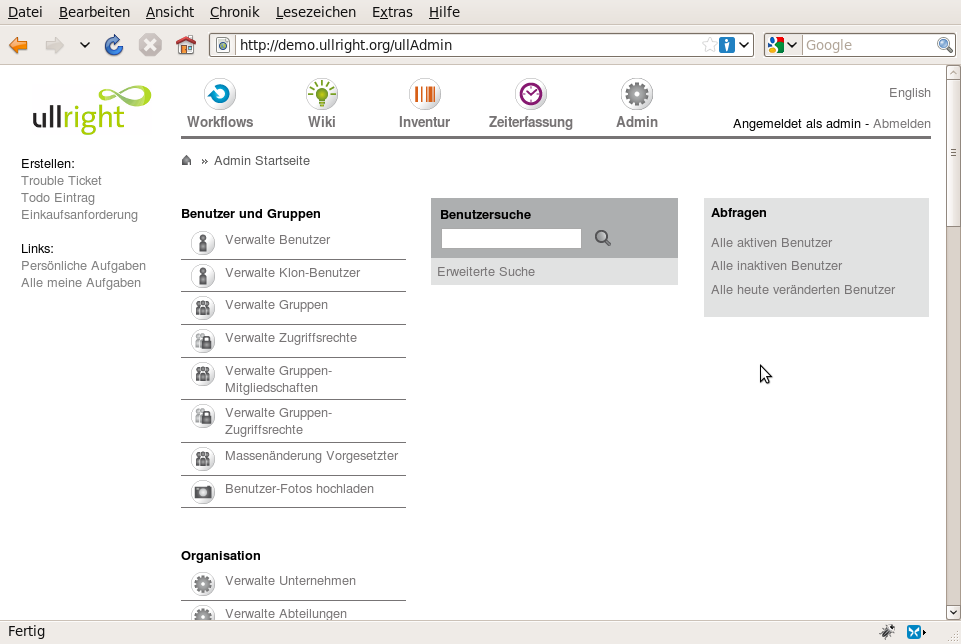
\includegraphics[width=0.9\textwidth]{figures/ullrightgermanexport-img8.png}
\caption{Der Administrationsbereich}
\label{fig:admin_index}
\end{figure}

Jedes ullright Modul, also auch die Administration, ist ähnlich aufgebaut, damit Sie sich schnell zurechtfinden.

Die Startseite (dargestellt in Abbildung \vref{fig:admin_index}) besteht aus drei Spalten. Diese sind, von links nach rechts:

\begin{itemize}
\item Aktionen
\item Suchfunktionen
\item Abfragen
\end{itemize}
Im Fall der Administration sind die Suchfunktionen und Abfragen speziell für die Benutzerverwaltung.

\subsection{Ergebnisliste}
Auch die Ergebnisliste hat eine einheitliche Bedienoberfläche für alle ullright Module.

Als Beispiel sehen wir uns (in Abbildung \vref{fig:user_result_list}) die Bedienung anhand der Benutzerverwaltung an.

\begin{figure}[htp]
\centering
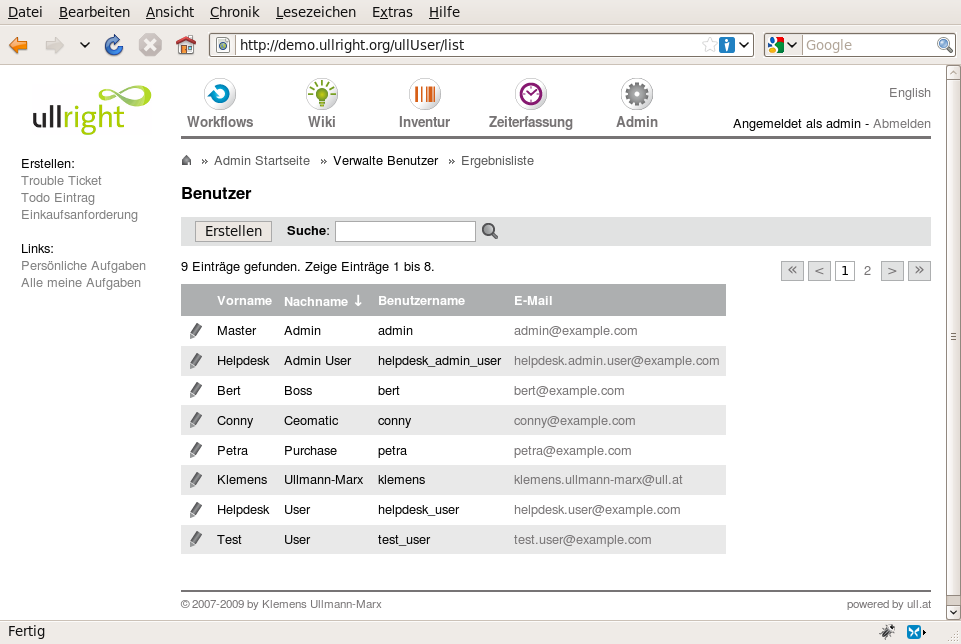
\includegraphics[width=0.9\textwidth]{figures/ullrightgermanexport-img9.png}
\caption{Die Benutzerverwaltung-Ergebnisliste}
\label{fig:user_result_list}
\end{figure}
Die Funktionen im Überblick:

\paragraph{Aktions / Filterleiste}
\begin{itemize}
\item Durch einen Klick auf "`Erstellen"' legen Sie einen neuen Eintrag an.
\item Das Suchfeld durchsucht bestimmte Felder.
\end{itemize}
\paragraph{Anzahl der Ergebnisse / Blättern}
\begin{itemize}
\item Sie sehen die Gesamtanzahl der gefundenen Einträge.
\item Bei mehr als 30 Einträgen (konfigurierbar) werden die Ergebnisse auf mehrere Seiten aufgeteilt. Es wird angezeigt welche Einträge man auf der aktuellen Seite sieht. Beispiel: "`Zeige Einträge 1 bis 30."'
\item Ganz rechts befindet sich die Funkton "`blättern"'. Erklärung der Symbole von links nach rechts:

\begin{itemize}
\item "`{\textless}{\textless}"' - zur ersten Seite springen
\item "`{\textless}"' - eine Seite zurückblättern
\item "`1"', "`2"', \ldots zur Seite n springen. Zeigt gleichzeitig die Zahl der Seiten
\item "`{\textgreater}"' - eine Seite vorblättern
\item "`{\textgreater}{\textgreater}"' - zur letzten Seite springen
\end{itemize}
\end{itemize}
\paragraph{Kopfzeile der Ergebnisliste}
Klicken Sie auf eine der Spaltenüberschriften, um danach zu sortieren. Klicken Sie ein weiteres Mal, um die Sortierreihenfolge umzukehren. Der Pfeil neben einer Spalte zeigt nach welcher Spalte sortiert wird und die Sortierrichtung.

\paragraph{Ergebnisliste -- Bearbeiten und Löschen}
Am Anfang jeder Zeile befinden sich die Aktionssymbole. Das Papierkorbsymbol bedeutet "`Löschen"', das Stiftsymbol bedeutet "`Bearbeiten"'. Das Löschen ist in manchen Fällen nicht möglich.

\paragraph{Tipp: Die Browser Adresszeile als Kommandozeile}
Alle ullright Module unterstützen aktiv das sogenannte "`Deep Linking"'. Das bedeutet, dass alle wichtigen Parameter, wie zum Beispiel ein Suchbegriff, in der Adressleiste angeführt sind.

Sie können somit jederzeit eine ullright-Adresse als Favorit in Ihrem Browser speichern oder einer Kollegin als Link per E-Mail schicken.

Beispiel: \url{http://demo.ullright.org/ullUser/list/filter[search]/example}

Zeigt alle Benutzer mit dem Suchbegriff "`example"'.

Ausnahme: für die erweiterte Suche steht diese Funktion nicht zur Verfügung.

\subsection{Erstellen}
Klicken Sie in der Ergebnisliste auf "`Erstellen"' um einen neuen Eintrag anzulegen, siehe Abbildung \vref{fig:create_user}.

\begin{figure}[htp]
\centering
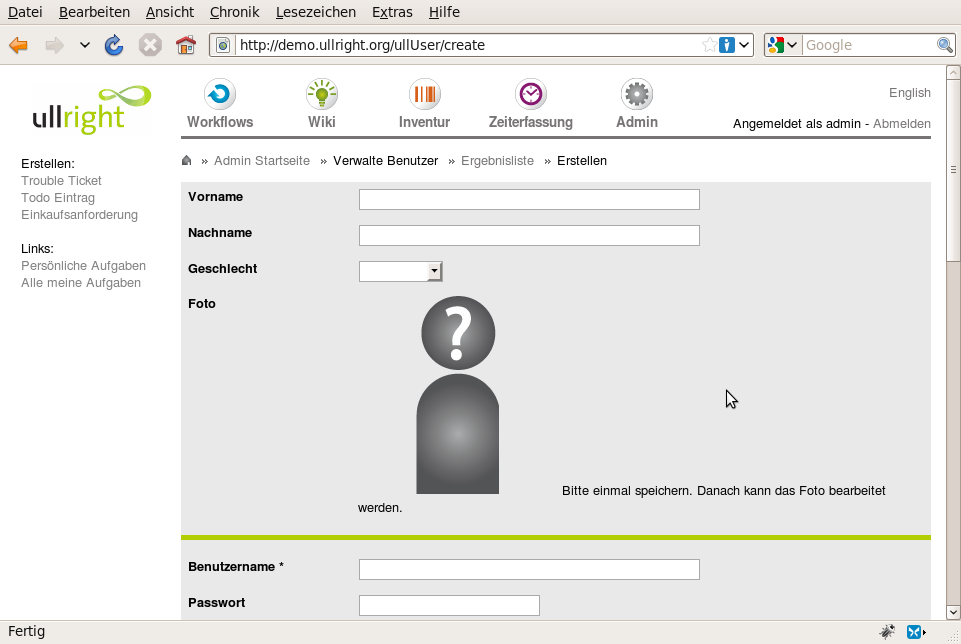
\includegraphics[width=0.9\textwidth]{figures/ullrightgermanexport-img10.png}
\caption{Ansicht "Benutzer anlegen"'}
\label{fig:create_user}
\end{figure}

Jedes Datenfeld befindet sich in einer eigenen Zeile. Links steht der Name des Feldes (z.B. Vorname), in der nächsten Spalte befindet sich das Eingabefeld. Wenn Sie nur Lesezugriff auf ein Feld haben wird kein Eingabefeld angezeigt. In der dritten Spalte werden etwaige Fehlermeldungen angezeigt (z.B. "`Pflichtfeld"' - siehe unten). 

Jedes Feld hat einen bestimmten Feldtyp, der bestimmt wie das Eingabefeld aussieht, und welche Eingaben  zulässig sind (Validierung). 

Pflichtfelder werden durch einen Stern * nach dem Feldnamen markiert (z.B. Benutzername).

Mehrsprachige Felder erkennen Sie an der Endung mit dem Sprachkürzel. Beispiel "`Beschriftung EN"'. Geben Sie Übersetzungen für alle aktivierten Sprachen ein.

Wenn Sie mit der Dateneingabe fertig sind klicken Sie auf "`Speichern"', siehe Abbildung \vref{fig:save_button}.

\begin{figure}[htp]
\centering
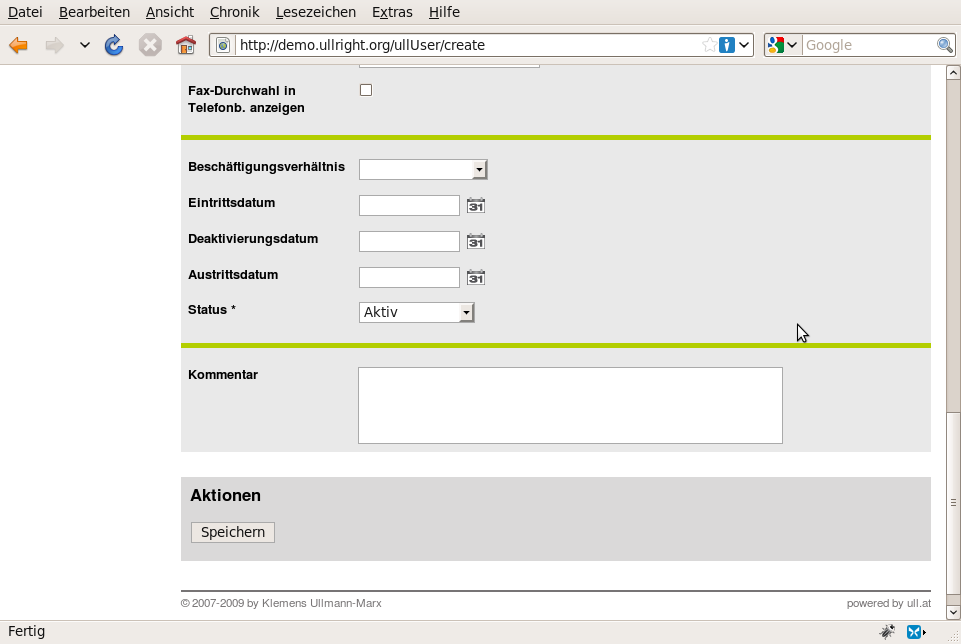
\includegraphics[trim=0 0 0 300pt,clip,width=0.9\textwidth]{figures/ullrightgermanexport-img11.png}
\caption{Der Speichern-Button}
\label{fig:save_button}
\end{figure}

Sie kehren nun zur letzten Ergebnislistenansicht zurück. 

\paragraph{Fehlerbehandlung}

Wenn Pflichtfelder nicht ausgefüllt werden, oder ungültige Werte eingegeben werden (z.B. ungültige E-Mailadresse) werden Sie darauf hingewiesen, dass Fehler aufgetreten sind (siehe Abbildung \vref{fig:validation_error}). Korrigieren Sie die markierten Eingaben und speichern Sie erneut.

\begin{figure}[htp]
\centering
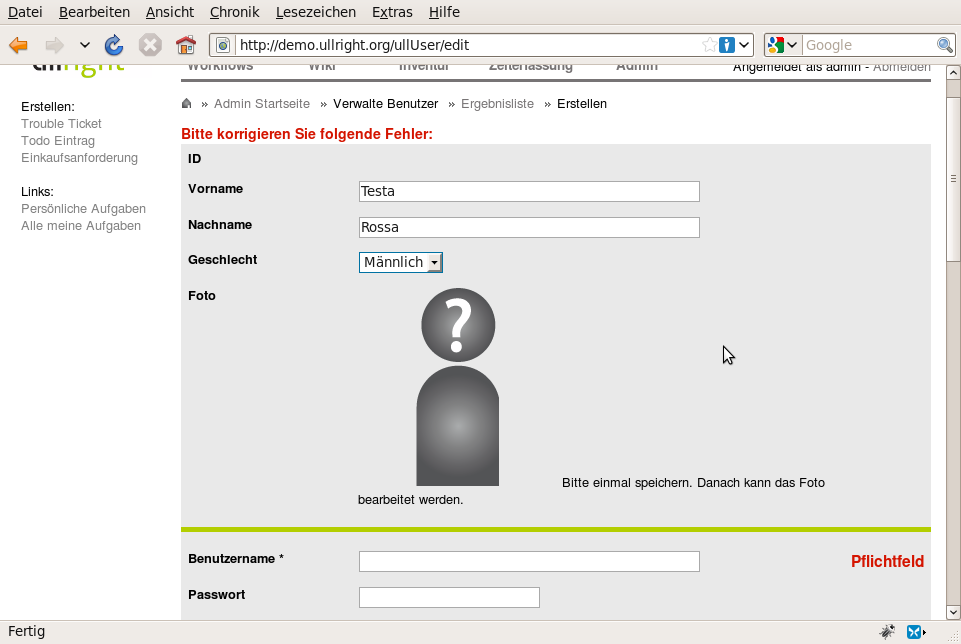
\includegraphics[width=0.9\textwidth]{figures/ullrightgermanexport-img12.png}
\caption{Hinweis auf fehlerhafte Eingabe}
\label{fig:validation_error}
\end{figure}

\subsection{Bearbeiten}
Die Bearbeitungsansicht ist der Ansicht "`Erstellen"' sehr ähnlich. Daher werden im folgenden nur die Unterschiede behandelt.

Es werden nun folgende Felder zusätzlich angezeigt:

\begin{enumerate}
\item Erstellt von
\item Erstellt am
\item Zuletzt aktualisiert von
\item Zuletzt aktualisiert am
\end{enumerate}
\subsection{Löschen}
Klicken Sie in der Ergebnisliste auf das Papierkorb-Symbol des gewünschten Eintrags.

\section{Auswahlfelder}
Sie können benutzerdefinierte Auswahlfelder anlegen und bearbeiten.

Benutzen Sie "`Verwalte Auswahlfelder"' um ein neues Auswahlfeld anzulegen.

Verwenden Sie danach "`Verwalte Auswahlfeld-Einträge"' um die Einträge der Liste anzulegen oder zu bearbeiten. Über das Feld "`Reihenfolge"' können sie manuell die Reihenfolge bestimmen.
\end{document}